% -------------------------------------------------------------------------------- %

\begin{exercise}[\textbf{Rolling die}]

A $d$-sided die with colored sides was rolled $n$ times.
The outcomes are stored in the file \texttt{die.Rdata} (each side appeared at least once).

\begin{enumerate}[label = (\alph*)]
    \item Visualize the relative frequencies in a colored barplot and add
    the standard error of each frequency. Given your graphic, what is your
    opinion on the assertion: 'the die is fair'?
    \item Test the null hypothesis that the die is fair with a $\chi^2$-test
    on the 5\%-significance level (without \texttt{chisq.test()})

    \begin{enumerate}[label = \roman*.]
        \item What are the observed (absolute) frequencies?
        What are the expected frequencies under the null hypothesis?
        \item What is the value $x^2$ of the $\chi^2$-statistic?
        How is the $\chi^2$-statistic $X^2$ distributed under the null
        hypothesis (in the context of the associated model).
        \item What is the rejection area? Do you reject the null hypothesis?
        \item Compute the $p$-value and interpret your result.
    \end{enumerate}

    \item Test the null hypothesis that the side 'orange' appears twice as
    often as the other sides (which appear with the same probability),
    on the 10\%-significance level.

    \begin{enumerate}[label = \roman*.]
        \item From the output of \texttt{chisq.test()} read the value
        of the $\chi^2$-statistic and the $p$-value.
        \item Can you reject the null hypothesis?
        \item Based on your calculations someone claims that the die is not
        loaded (i.e., it is fair). What do you answer the person?
    \end{enumerate}
\end{enumerate}

\end{exercise}

% -------------------------------------------------------------------------------- %

\begin{solution}

\phantom{}

\begin{enumerate}[label = (\alph*)]


    \item 

    \begin{figure}[H]
        \centering
        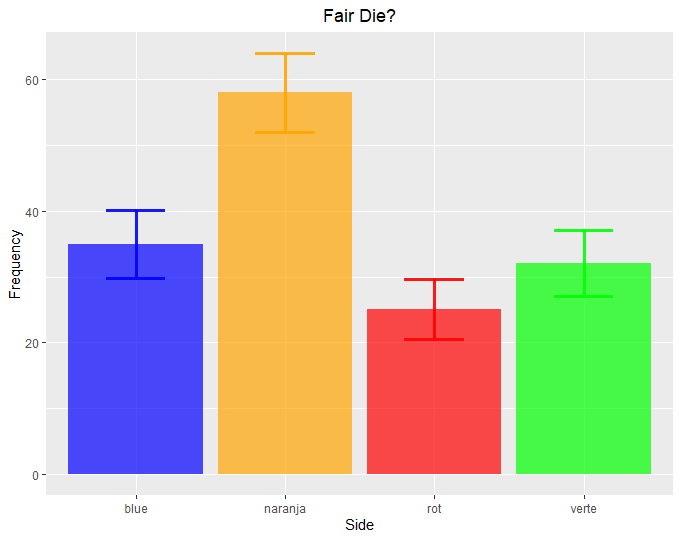
\includegraphics[width = 0.8 \textwidth]{13.3.barplot.png}
    \end{figure}
    Based on the graphical representation of the observed frequencies
    I would guess that the die is biased towards \textit{naranja}.

    \item In our case we have $n = 150$. The observed and expected 
    frequencies under the null are:
    
    \begin{center}
    \begin{tabular}{c|c|c}
        Side & Observed & Expected \\
        \hline
        Blue & 35 & 37.5 \\
        Naranja & 58 & 37.5 \\
        Rot & 25 & 37.5 \\
        Verte & 35 & 37.5
    \end{tabular}
    \end{center}

    Calculating the value of the $X^2$-statistic yields

    \begin{align*}
        X^2 = \frac{2.5^2+20.5^2+12.5^2+2.5^2}{35} \approx 16.83.
    \end{align*}

    Since we know that under the null $X^2 \sim \chi^2(3)$,
    the rejection region at $\alpha = 0.05$ reads

    \begin{align*}
        R = [\chi^2_{\alpha}(3),\infty[ \approx [7.81,\infty[.
    \end{align*}

    Based on the rejection region we reject the null hypothesis that the die is fair.

    Computing the $p$-value yields

    \begin{align*}
        p-\text{value} = \P(X^2 > 16.83) = 0.0007659755 < 0.05,
    \end{align*}

    which agrees with the previous result.

    \item \texttt{chisq.test()} gives the following result:
    
    \begin{lstlisting}
        X-squared = 1.8667, df = 3, p-value = 0.6005
    \end{lstlisting}

    Based on these results we cannot reject the null hypothesis.
    However, this does not conclusively prove the null hypothesis that the die is fair,
    it merely states that there is insufficient evidence to definitively say that the dice is loaded.
\end{enumerate}

\end{solution}

% -------------------------------------------------------------------------------- %
